\documentclass[letterpaper, 12pt]{article}

\usepackage{hyperref}
\usepackage{pgfplots}
\usepgfplotslibrary{fillbetween}


\title{Basics of Economics}
\author{Alvin Lin}
\date{Principles of Microeconomics: August 2016 - December 2016}

\begin{document}

\maketitle

\section{Global Markets}
International trade is driven by comparative advantages. A nation has a
comparative advantage in producing a good if it can produce it at a lower
opportunity cost than any other nation.

\subsection{Markets with Imports}
If the world price is less than the domestic equilibrium price, imports will
occur. Domestic consumers benefit from this while producers are harmed by this.
However, there is a net gain.

\subsection{Markets with Exports}
If the world price is greater than the domestic equilibrium price, exports will
occur. Domestic consumers are harmed by this while producers benefit from this.
There is a net gain overall.

\subsection{Protecting Domestic Producers: Trade Restrictions}

\subsubsection{Tariffs}
A tariff is a tax imposed on imports by the importing country. For example,
India imposes a 100\% tariff on wine imported from California. Domestic
producers benefit from import tariffs while consumers are worse off. The
government gains tariff revenue, but there is a still a deadweight loss
because consumers lose more than the amount gained by producers and the
government.

\subsubsection{Import Quotas}
An import quota is a limit on the quantity that can be imported. For example,
the US imports quotas on dairy products, chocolate, cotton, and brooms.
Domestic producers benefit from import quotas while domestic producers are
worse off. Importers gain profit, but there is still a deadweight loss because
consumers lose more than the amount gained by producers and the government.

\subsubsection{A Comparison of Tariffs and Quotas}
Given a desired level of imports, the same price is paid by consumers, the same
quantity is traded, the same amount of produced by domestic suppliers, and there
is the same deadweight loss. With tariffs, the government gains revenue, while
with quotas, importers gain profit.

\subsubsection{Example}
\[ Q_{supplied\ domestic} = P \]
\[ Q_{demanded\ domestic} = 10-P \]
\[ P_{world} = 2 \]
\begin{center}
  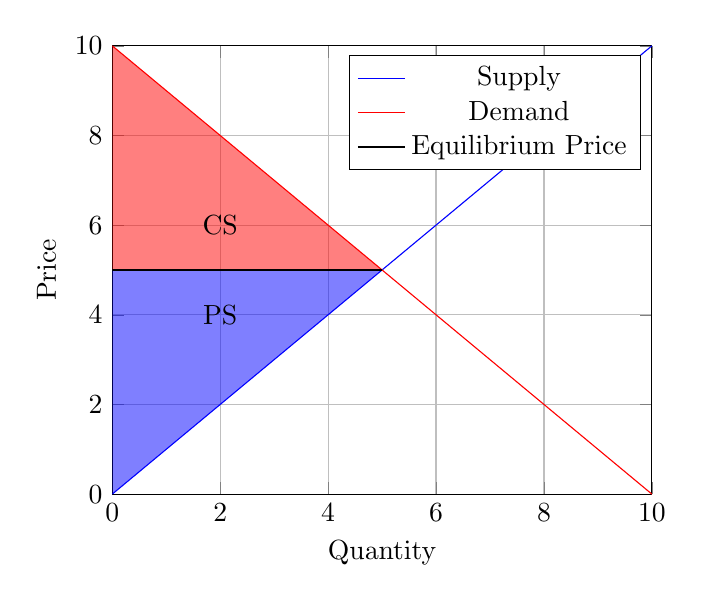
\begin{tikzpicture}
    \begin{axis} [
      xlabel={Quantity}, ylabel={Price},
      xmin=0, xmax=10, ymin=0, ymax=10,
      grid=both
    ]
      \addplot[name path=supply, color=blue] coordinates { (0,0) (10,10) };
      \addlegendentry{Supply};
      \addplot[name path=demand, color=red] coordinates { (0,10) (10,0) };
      \addlegendentry{Demand};
      \addplot[name path=equilibrium, color=black] coordinates { (0,5) (5,5) };
      \addlegendentry{Equilibrium Price};
      \addplot[color=blue, fill=blue, fill opacity=0.5]
        fill between [of=equilibrium and supply, soft clip={domain=0:5}];
      \addplot[color=red, fill=red, fill opacity=0.5]
        fill between [of=equilibrium and demand, soft clip={domain=0:5}];
      \node[draw=none] at (2,6) {CS};
      \node[draw=none] at (2,4) {PS};
    \end{axis}
  \end{tikzpicture}
\end{center}
\[ P^{*} = 10-P^{*} \]
\[ P^{*} = 5\ (\mathrm{equilibrium\ price}) \]
\begin{center}
  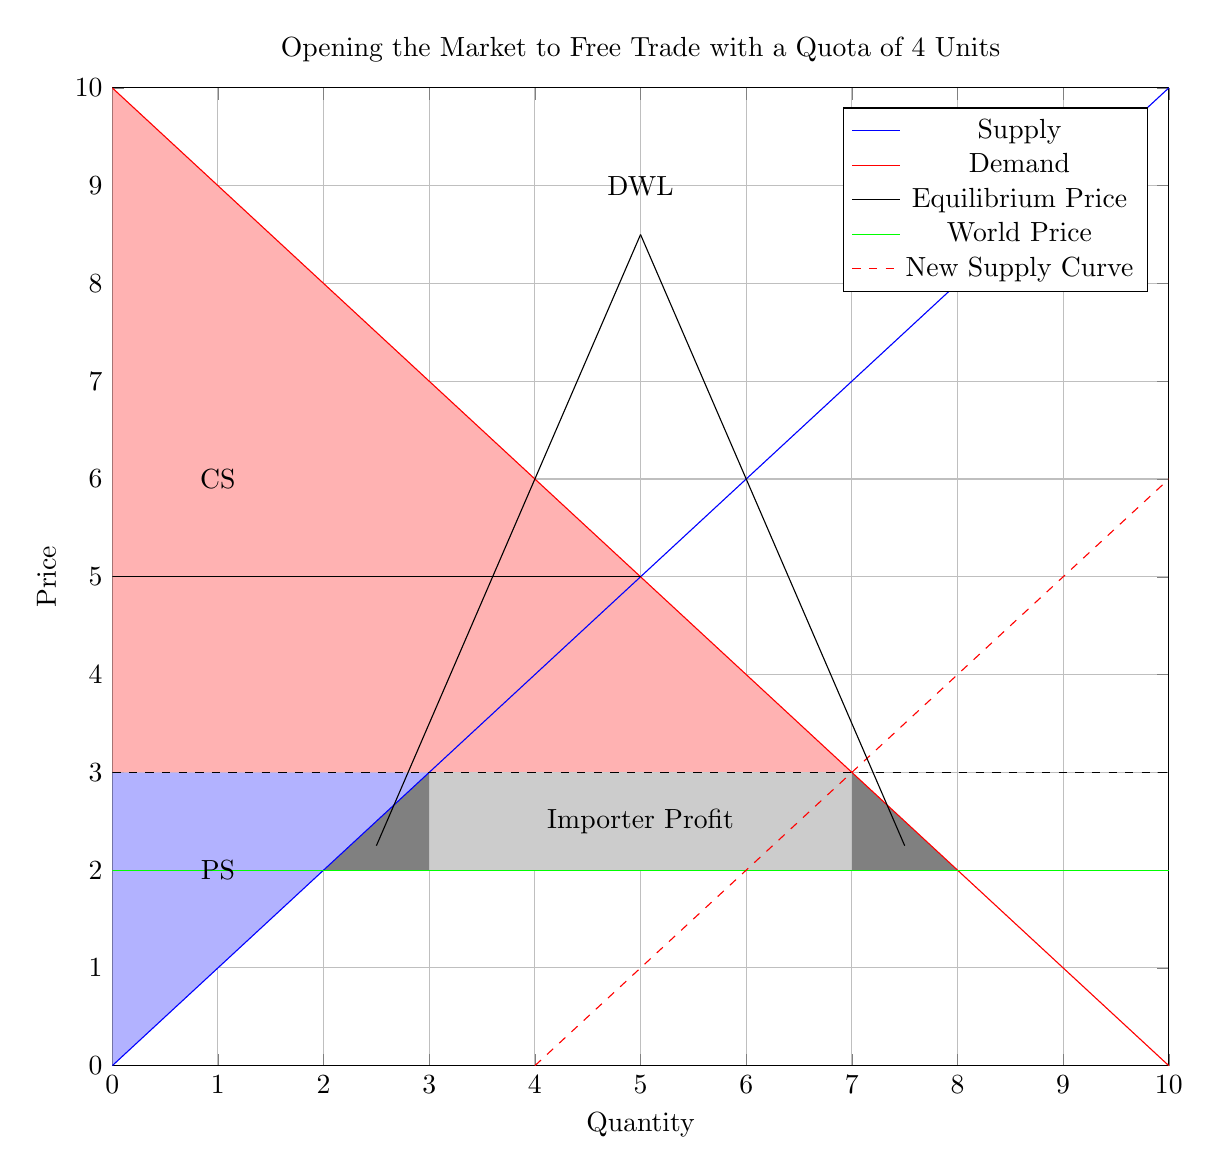
\begin{tikzpicture}
    \begin{axis} [
      xlabel={Quantity}, ylabel={Price},
      width=15cm, height=14cm,
      title={Opening the Market to Free Trade with a Quota of 4 Units},
      xtick={0,1,...,10}, ytick={0,1,...,10},
      xmin=0, xmax=10, ymin=0, ymax=10,
      grid=both
    ]
      \addplot[name path=supply, color=blue] coordinates { (0,0) (10,10) };
      \addlegendentry{Supply};
      \addplot[name path=demand, color=red] coordinates { (0,10) (10,0) };
      \addlegendentry{Demand};
      \addplot[name path=equilibrium, color=black] coordinates { (0,5) (5,5) };
      \addlegendentry{Equilibrium Price};
      \addplot[name path=world, color=green] coordinates { (0,2) (10,2) };
      \addlegendentry{World Price};
      \addplot[name path=supply2, color=red, dashed] coordinates
        { (4,0) (10,6) };
      \addlegendentry{New Supply Curve};
      \addplot[name path=equilibrium2, dashed] coordinates { (0,3) (10,3) };
      \addplot[color=blue, fill=blue!30]
        fill between [of=equilibrium2 and supply, soft clip={domain=0:3}];
      \addplot[color=red, fill=red!30]
        fill between [of=equilibrium2 and demand, soft clip={domain=0:7}];
      \addplot[color=black, fill=black!20]
        fill between [of=equilibrium2 and world, soft clip={domain=3:7}];
      \addplot[color=black, fill=black!50]
        fill between [of=world and supply, soft clip={domain=2:3}];
      \addplot[color=black, fill=black!50]
        fill between [of=world and demand, soft clip={domain=7:8}];
      \node[draw=none] at (1,6) {CS};
      \node[draw=none] at (1,2) {PS};
      \node at (5,9) {DWL};
      \addplot[color=black] coordinates { (2.5,2.25) (5,8.5) };
      \addplot[color=black] coordinates { (7.5,2.25) (5,8.5) };
      \node[draw=none] at (5,2.5) {Importer Profit};
    \end{axis}
  \end{tikzpicture}
\end{center}
\[ 4 + P^{**} = 10-P^{**} \]
\[ 2P^{**} = 6 \]
\[ P^{**} = 3 \]

\subsection{Common Arguments For/Against Trade Restrictions}
\begin{itemize}
  \item Argument: They help infant industries grow.
  \item Counter-argument: They also protect firms that are not producing
  efficiently.
  \item Argument: They counteract dumping.
  \item Counter-argument: Dumping is very hard to detect because it
  is hard to know a firm's costs. A low price might be set by a producer
  because she faces elastic demand.
  \item Argument: They save domestic jobs.
  \item Counter-argument: They might create jobs in one sector and destroy
  jobs in another.
  \item Argument: They allow us to compete with cheap foreign labor.
  \item Counter-argument: Wages are determined by productivity. High
  productivity workers get higher wages and low productivity workers get lower
  wages.
  \item Argument: They protect rich countries from exploiting poor ones.
  \item Counter-argument: By trading with poor countries, we increase the
  demand for their labor and increase their income.
\end{itemize}

\begin{center}
  You can find all my notes at \url{http://omgimanerd.tech/notes}. If you have
  any questions, comments, or concerns, please contact me at
  alvin@omgimanerd.tech
\end{center}

\end{document}
